\documentclass[a4paper]{article}

%% Language and font encodings
%\usepackage{fontspec}
%\setmainfont{Times New Roman}\usepackage{CormorantGaramond}
\usepackage[toc,page]{appendix}
\usepackage[T1]{fontenc}
\usepackage[utf8x]{inputenc}
\usepackage[swedish, english]{babel}
\usepackage{float}
\usepackage[colorlinks=true, allcolors=black]{hyperref}
\usepackage[dvipsnames]{xcolor}
\usepackage{tikz}
\usepackage{circuitikz} % for circuit diagrams
\usepackage{caption}
\usepackage{subcaption}
\usepackage{graphicx}
\usepackage{mathtools}
\urlstyle{tt}
\newcommand{\email}[1]{\href{mailto:#1}{\tt{\nolinkurl{#1}}}}
\newcommand{\orcid}[1]{ORCID: \href{https://orcid.org/#1}{\tt{\nolinkurl{#1}}}}

\usepackage[parfill]{parskip}
\renewcommand*\oldstylenums[1]{\carlitoOsF #1}
% \usepackage{fancyhdr}
%\usepackage{natbib}
\usepackage{authblk}
\setlength{\headheight}{41pt}
\setlength{\textwidth}{440pt}
%\pagestyle{fancy}

%% Sets page size and margins
\usepackage[a4paper,top=3cm,bottom=2cm,left=3cm,right=3cm,marginparwidth=1.75cm]{geometry}

%% Useful packages
\usepackage{graphicx}
\usepackage{booktabs}
%\usepackage{caption}
\usepackage{amsmath}
\usepackage{mathtools}
\usepackage{titlesec}
\setcounter{secnumdepth}{4}

\usepackage[colorinlistoftodos]{todonotes}
\usepackage[yyyymmdd]{datetime}
\renewcommand{\dateseparator}{-}
\rmfamily
% \fancyhead[L]{\rmfamily Bi-MMC battery}

\usepackage{xspace}
\def\id{\textit{i\textsubscript{d}}\xspace} % id
\def\iq{\textit{i\textsubscript{q}}\xspace} % iq
\def\Te{\textit{T\textsubscript{e}}\xspace} % Te

\def\vd{\textit{v\textsubscript{d}}\xspace} % vd
\def\vq{\textit{v\textsubscript{q}}\xspace} % vq

\def\ia{\textit{i\textsubscript{a}}\xspace} % ia
\def\ib{\textit{i\textsubscript{b}}\xspace} % ib
\def\ic{\textit{i\textsubscript{c}}\xspace} % ic

\def\va{\textit{v\textsubscript{a}}\xspace} % va
\def\vb{\textit{v\textsubscript{b}}\xspace} % vb
\def\vc{\textit{v\textsubscript{c}}\xspace} % vc

\def\ialpha{\textit{i\textsubscript{$\alpha$}}\xspace} % ialpha
\def\ibeta{\textit{i\textsubscript{$\beta$}}\xspace} % ibeta

\def\valpha{\textit{v\textsubscript{$\alpha$}}\xspace} % valpha
\def\vbeta{\textit{v\textsubscript{$\beta$}}\xspace} % vbeta

\def\we{\textit{$\omega_{\textit{e}}$}\xspace} % we
\def\wm{\textit{$\omega_{\textit{m}}$}\xspace} % wm

\def\J{\textit{J}\xspace} % J
\def\np{\textit{n\textsubscript{p}}\xspace} % number of pole pairs
\def\Nr{\textit{N\textsubscript{r}}\xspace} % motor speed in RPM
\def\Nrnom{\textit{N\textsubscript{r(nom)}}\xspace} % nominal motor speed
\def\Ld{\textit{L\textsubscript{d}}\xspace} % Ld
\def\Lq{\textit{L\textsubscript{q}}\xspace} % Lq
\def\Rs{\textit{R\textsubscript{s}}\xspace} % iq
\def\flux{\textit{$\Psi$}\xspace} % flux constant

\def\is{\textit{i\textsubscript{s}}\xspace} % stator current

\def\Tl{\textit{T\textsubscript{l}}\xspace} % load torque

%\def\iqq{\textit{i\textsubscript{q}}\xspace} % iq


% \usepackage[utf8]{inputenc}
\usepackage{prettyref}
\newrefformat{fig}{Figure \ref{#1}}
\newrefformat{tab}{Table \ref{#1}}

% package for text width 
\usepackage{layouts}

%% Package to import MATLAB codes
\usepackage{listings}
%\usepackage[usenames,dvipsnames]{color}

% This is the color used for MATLAB comments below
%\definecolor{MyDarkGreen}{rgb}{0.0,0.4,0.0}

% For faster processing, load Matlab syntax for listings
%\lstloadlanguages{Matlab}%
\definecolor{codegreen}{rgb}{0,0.6,0}
\definecolor{codegray}{rgb}{0.5,0.5,0.5}
\definecolor{codepurple}{rgb}{0.58,0,0.82}
\definecolor{mygreen}{RGB}{28,172,0} 
\definecolor{mylilas}{RGB}{170,55,241}
\definecolor{backcolour}{rgb}{0.95,0.95,0.92}
	
\lstdefinestyle{mystyle}{
	backgroundcolor=\color{backcolour},   
	commentstyle=\color{codegreen},
	keywordstyle=\color{blue},
	numberstyle=\tiny\color{codegray},
	stringstyle=\color{codepurple},
	basicstyle=\ttfamily\scriptsize,
	breakatwhitespace=false,         
	breaklines=true,                 
	captionpos=b,                    
	keepspaces=true,                 
	numbers=left,                    
	numbersep=5pt,                  
	showspaces=false,                
	showstringspaces=false,
	showtabs=false,                  
	tabsize=2,
	aboveskip=\medskipamount
}
\lstset{style=mystyle,language=MATLAB}

%\lstset{ 
%	language=Matlab,                		% choose the language of the code
%	%	basicstyle=10pt,       				% the size of the fonts that are used for the code
%	numbers=left,                  			% where to put the line-numbers
%	numberstyle=\footnotesize,      		% the size of the fonts that are used for the line-numbers
%	stepnumber=1,                   			% the step between two line-numbers. If it's 1 each line will be numbered
%	numbersep=5pt,                  		% how far the line-numbers are from the code
%	%	backgroundcolor=\color{white},  	% choose the background color. You must add \usepackage{color}
%	showspaces=true,               		% show spaces adding particular underscores
%	showstringspaces=true,         		% underline spaces within strings
%	showtabs=true,                 			% show tabs within strings adding particular underscores
%	%	frame=single,	                			% adds a frame around the code
%	%	tabsize=2,                				% sets default tabsize to 2 spaces
%	%	captionpos=b,                   			% sets the caption-position to bottom
%	breaklines=true,                			% sets automatic line breaking
%	breakatwhitespace=false,        		% sets if automatic breaks should only happen at whitespace
%	escapeinside={\%*}{*)}          		% if you want to add a comment within your code
%}

\title{\Large Simulation of a Permanent Magnet Synchronous Machine}
\author{Arvind Balachandran}
\date{\today}

\begin{document}
	
	\maketitle
	\pagenumbering{gobble}
	\newpage
	\pagenumbering{arabic}
	\begin{center}
		\fbox{\begin{minipage}[h!]{\textwidth}
				\centering
				The aim of the project is to simulate an electric machine and show that the numerical solution gives the same solution as the differential equation.
		\end{minipage}}
	\end{center}
	\section{PMSM Model}
This section presents the model of a PMSM electric machine. 

Instantaneous three-phase voltages (\va, \vb, and \vc) and currents (\ia, \ib , and \ic) can be written as follows:
\begin{align*}
	\va(t) &= \hat\va\,\cos\left(\we\,t\right), & \vb(t) &= \hat\vb\,\cos\left(\we\,t + \frac{2\,\pi}{3}\right), & \vc(t) &= \hat\vc\,\cos\left(\we\,t - \frac{2\,\pi}{3}\right), \\
	\ia(t) &= \hat\ia\,\cos\left(\we\,t - \phi\right), & \ib(t) &= \hat\ib\,\cos\left(\we\,t + \frac{2\,\pi}{3} - \phi\right), & \ic(t) &= \hat\ic\,\cos\left(\we\,t - \frac{2\,\pi}{3} - \phi\right).
\end{align*}
Assuming a balanced 3-phase network, i.e:
\begin{align*}
	\va + \vb + \vc &= 0, & \ia + \ib + \ic &=0
\end{align*}
Transformation to an equivalent two-phase system, i.e, Clarke transformation, is presented as follows: 
\begin{align*}
	\begin{pmatrix}
		\valpha \\
		\vbeta
	\end{pmatrix} &= \frac{2\,K}{3} \begin{pmatrix}
										1 & -\frac{1}{2} & -\frac{1}{2} \\
										0 & \frac{\sqrt3}{2} & -\frac{\sqrt{3}}{2} \\
									\end{pmatrix}\, \begin{pmatrix}
														\va \\
														\vb \\
														\vc
													\end{pmatrix}, & 	\begin{pmatrix}
													\ialpha \\
													\ibeta
												\end{pmatrix} &= \frac{2\,K}{3} \begin{pmatrix}
												1 & -\frac{1}{2} & -\frac{1}{2} \\
												0 & \frac{\sqrt3}{2} & -\frac{\sqrt{3}}{2} \\
											\end{pmatrix}\, \begin{pmatrix}
											\ia \\
											\ib \\
											\ic
										\end{pmatrix},
\end{align*}
where $K$ is a constant (1, peak-scaling and $\sqrt{3/2}$ for power-scaling).

In-order to simplify the analysis, the reference frame of a three-phase vectors are rotated. i.e:
\begin{align*}
	\begin{pmatrix}
			\vd \\
			\vq
	\end{pmatrix} &= \begin{pmatrix}
						\cos(\we\,t) & -\sin(\we\,t) \\
						\sin(\we\,t) & \cos(\we\,t) \\
					 \end{pmatrix}\, \begin{pmatrix}
										 \valpha \\
										 \vbeta
									 \end{pmatrix} & \begin{pmatrix}
									 \id \\
									 \iq
								 \end{pmatrix} &= \begin{pmatrix}
								 \cos(\we\,t) & -\sin(\we\,t) \\
								 \sin(\we\,t) & \cos(\we\,t) \\
							 \end{pmatrix}\, \begin{pmatrix}
							 \ialpha \\
							 \ibeta
						 \end{pmatrix}
\end{align*}
The PMSM can thus be modeled as follows:
\begin{align*}
	\Ld\,\frac{d\id}{dt} &= \vd - \Rs\,\id + \Lq\,\iq\,\wm,\\
	\Lq\,\frac{d\iq}{dt} &= \vq - \Rs\,\iq - \left(\Ld\,\id + \flux\right)\,\wm,\\
	\J\,\frac{d\wm}{dt} &= \frac{3\,\np}{2\,K^2}\,\left(\left(\Ld - \Lq\right)\,\id\,\iq + \iq\,\flux\right) - \Tl,
\end{align*}
where \wm is PMSM rotor rotating magnetic field's angular velocity, \Rs is the stater resistance per phase, \Ld and \Lq are $d$ and $q$ axis inductances, respectively, \flux is the flux constant of the permanent magnet, \np is the number of pole pairs, and \Tl is the load torque. 

\fbox{\begin{minipage}[h!]{\textwidth}
	The system equations are given below:
	\begin{align}
		\va &= \hat\va\,\cos(\we\,t), & (\text{input}),\\
		\vb &= \hat\vb\,\cos(\we\,t + \frac{2\,\pi}{3}), & (\text{input}),\\
		\vc &= \hat\vc\,\cos(\we\,t - \frac{2\,\pi}{3}), & (\text{input}),\\
	%% --- alpha beta
		\valpha &= \frac{2\,K}{3}\,\left(\va -\frac{1}{2}\,\vb -\frac{1}{2}\,\vc\right), \\
		\vbeta &= \frac{2\,K}{3}\,\left(\frac{\sqrt3}{2}\,\vb -\frac{\sqrt3}{2}\,\vc\right), \\
	%% --- dq
		\vd &= \cos(\we\,t)\,\valpha - \sin(\we\,t)\,\vbeta,\\
		\vq &= \sin(\we\,t)\,\valpha + \cos(\we\,t)\,\vbeta,\\ 
%		\begin{pmatrix}
%			\vd \\
%			\vq
%		\end{pmatrix} &= \begin{pmatrix}
%			\cos(\we\,t) & -\sin(\we\,t) \\
%			\sin(\we\,t) & \cos(\we\,t) \\
%		\end{pmatrix}\, \begin{pmatrix}
%			\valpha \\
%			\vbeta
%		\end{pmatrix} \\
	%% --- state equations
		\Ld\,\frac{d\id}{dt} &= \vd - \Rs\,\id + \Lq\,\iq\,\wm,\\
		\Lq\,\frac{d\iq}{dt} &= \vq - \Rs\,\iq - \left(\Ld\,\id + \flux\right)\,\wm,\\
		\J\,\frac{d\wm}{dt} &= \frac{3\,\np}{2\,K^2}\,\left(\left(\Ld - \Lq\right)\,\id\,\iq + \iq\,\flux\right) - \Tl,\\
	%% --- output variables
		\is &= \id + j\,\iq, & (\text{output}),\\
		\Te &= \frac{3\,\np}{2\,K^2}\,\left(\left(\Ld - \Lq\right)\,\id\,\iq + \iq\,\flux\right), & (\text{output}),\\
		\Nr &= \frac{\wm}{\np}\,\frac{30}{\pi}, & (\text{output}).
	\end{align}
\end{minipage}}

The above gives the ODE with three dynamic variables, \id, \iq, \wm. 
	
The main aim of the project is to show that the numerical solution gives the same solution as the differential equation. However, we cannot determine the solution analytically. Therefore, we need to try perform the several checks. The following sections cover these in detail. 

Two different single step numerical methods are chosen: a fixed-step and a variables step length methods. \textit{Euler forward} method is used as the fixed step solver. The \textit{Dormand-Prince 4(5)} method is employed as the variable step length solver.

The table \prettyref{tab:simparam} below provides the simulation parameters:
\begin{table}[h!b!]
	\centering
	\begin{tabular}{c|c|c}
		Parameter Name & Parameter symbol & value \\
		\hline
		Peak input voltage & $\hat \va,\ \hat \vb,\ \hat \vc $ & 800\,V\\
		Load torque & \Tl & 0\\
		Motor inertia & \J & 1.09\,kgm$^2$\\
		Number of pole pairs & \np & 20\\
		Rated speed (Nominal speed) & \Nrnom & 1000\,rpm \\
		Electrical frequency & \textit{f\textsubscript{1}} & 166.67\,Hz\\
		Stator inductance (direct axis)& \Ld & 48.35\,$\mu$H\\
		Stator inductance (quadrature axis)& \Ld & 48.35\,$\mu$H\\
		Stator resistance & \Rs & 0.052 \\
		Flux constant & $\Psi$ & 0.38 \\
		Clarke Constant & $K$ & 1
	\end{tabular}
	\caption{Simulation parameters for the PMSM}
	\label{tab:simparam}
\end{table}

	\newpage
	\input{sections/sim.tex}
	% % \section{Fixed step solver}
% \subsection{Test Equation}
% \begin{figure}[h!]
% 	\centering
% 	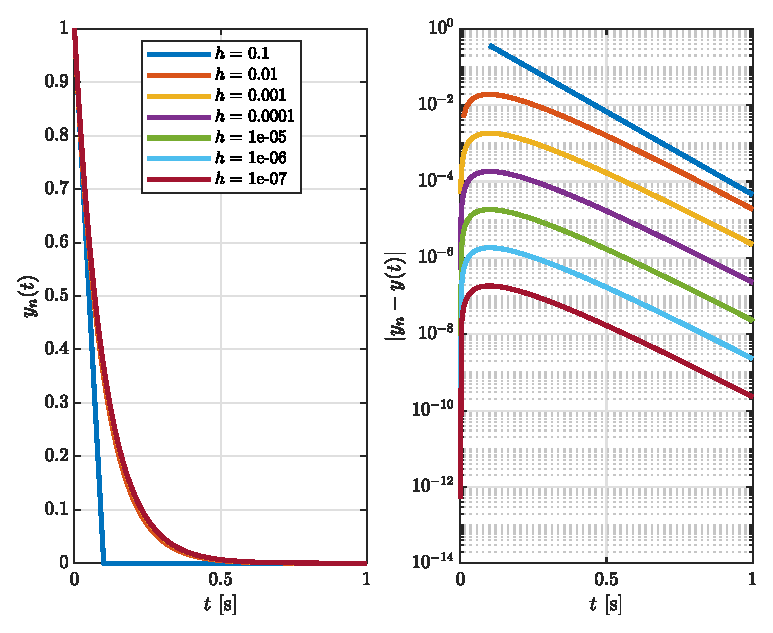
\includegraphics[width=\textwidth]{Figures/ef_testCase.eps}
% 	\caption{Simulation of the test equation using the Euler forward method with $\lambda=1$.}
% 	\label{fig:testEF}
% \end{figure}
% The consistency of the Euler forward method is checked by using a test equation. The test equation is given as follows:
% \begin{align*}
% 	\textbf{Test equation: }f(t,y) &= -\lambda\,y, \quad y(0) = 1. & \textbf{Analytical solution: } & y = e^{-\lambda\,t}.
% \end{align*}

% Using the test equation, the solver's (or numerical method's) \textit{convergence} is checked.

% \subsubsection{Convergence}
% The solver arrives at a solution that is close to the exact solution within some pre-specified error tolerance or other convergence criterion. This is the significance of convergence. % This is the, indeed,goal of the project. 

% By definition, the solver is said to be \textit{convergent of order $p$} if the global error $e_n$, satisfies
% \begin{align*}
% 	e_n = O(h^p)
% \end{align*}

% The simulation results of the test equation are presented in \prettyref{fig:testEF}. From the figure, the order of the system is calculated and presented in the table below:
% \begin{table}[h!]
% 	\centering
% 	\begin{tabular}{c|c|c}
% 		h & $|y_n - y(t)|$ & $p$ \\
% 		\hline
% 		0.1 & 1.58e-3 & \\
% 		0.01 & 1.67e-4 & 0.95\\
% 		0.001 & 1.68e-5 & 0.99 \\
% 		0.0001 & 1.68e-6 & 1 \\
% 		1e-5 & 1.69e-7 & 1 \\
% 		1e-6 & 1.69e-8 & 1 \\		
% 		1e-7 & 1.69e-9 & 1 	
% 	\end{tabular}
% \end{table}\\
% From the table and the figure, it is clear that, as $h\rightarrow0,\ |y_n - y(t)| \rightarrow0$. Therefore, according to the fundamental convergence theorem, the solver is \textit{convergent of order $p$}. % Furthermore, is can also be observed that the solver is also \textit{consistent} and also \textit{0-stable}. 

\subsection{Simulation with fixed-step solver}
\begin{figure}[t!b!]
	\centering
	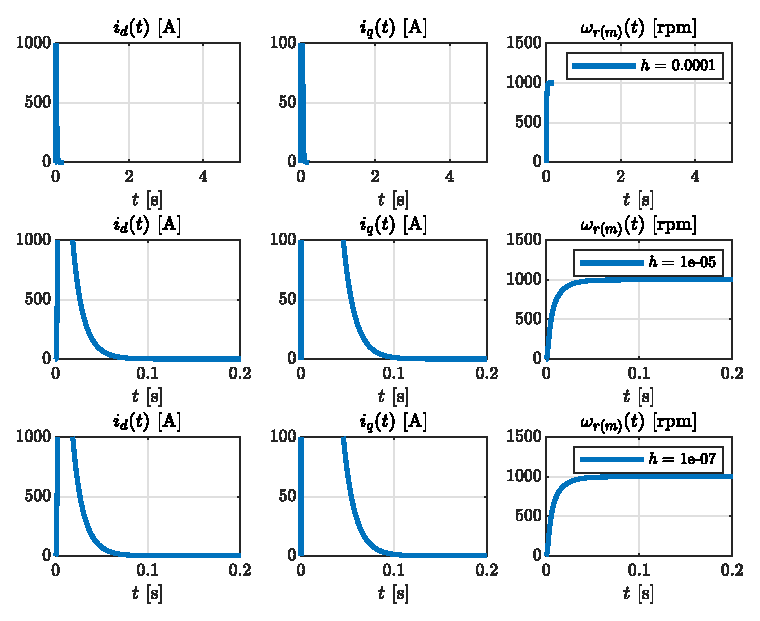
\includegraphics[width=\textwidth]{Figures/ef_MotorCase.eps}
	\caption{Simulation of the PMSM using Euler forward method with $\vd=\vq=800\,$V at three different step sizes, $h = 0.001$, $h = 1\text{e}-5$, and $h = 1\text{e}-7$ .}
	\label{fig:EMresEF}
\end{figure}
\prettyref{fig:EMresEF} presents the simulation results of a PMSM using the \textit{forward Euler} method. The figure shows the states (dynamic variables) \id, \iq, and \wm as a function of time. From the figure, it is clear that as $h \rightarrow 0$. all the states converge to a constant value. The time constant of the current transient (\Ld/\Rs) is about $9.9\text{e}-4$\,s. The minimum step size should be below this for the solver to converge. 

\fbox{\parbox{0.98\textwidth}{
\emph{When should one use $h = 1\text{e}-5$, and $h = 1\text{e}-7$?} \\
if the goal is to analyze the steady state of the speed, i.e., after 0.5\,s, then $h = 1\text{e}-5$ is sufficient. If the goal is to get very accurate information about the current transient, lower $h$ is better.

\emph{Why can we trust the results?} \\
As $h \rightarrow 0$, the current transient peak and the time constant reaches closer to (\Ld/\Rs) is about $9.9\text{e}-4$\,s. Furthermore, the errors both during the transients and steady states reduce as $h \rightarrow 0$. Therefore, we can trust the results, because they align with the theory of \textit{convergence}, as $h \rightarrow 0$, the numerical solutions are close to the true solution. 
}}

% This implies that % that the solver is \textit{0-stable}. Furthermore, it is also clear that 
% the ODE system is stable. 

% The \textit{convergence} of the numerical method was checked in the previous section. Therefore, it can be concluded that the simulated results with $h \leq 1\text{e}-4$ gives the a solution that is very close to the true solution to the ode system.

%\subsubsection{Validation from control theory}
%During steady state operation on the PMSM, i.e, 1\,s simulation time, the \texttt{odes} (8), (9), and (10) can be simplified, as follows:
%\begin{align}
%	\Rs\,\id - \vd &= \Lq\,\iq\,\wm, & \vq - \Rs\,\iq &= \left(\Ld\,\id + \flux\right)\,\wm, & \Tl\,\frac{2\,K^2}{3\,\np} &= \iq\,\left(\left(\Ld - \Lq\right)\,\id + \flux\right), \label{eq:simlified}
%\end{align}
%Substituting the initial conditions for the simulation in \prettyref{eq:simlified}, we get:
%\begin{align*}
%	\iq &= 0
%\end{align*}

%The error at $t_N$ is given in the table below:
%\begin{table}[h!]
%	\centering
%	\begin{tabular}{c|c|c|c}
%		h & $|\id_N + j\,\iq_N|$ & \Te\textsubscript{\textit{N}} & \Nr\textsubscript{\textit{N}}\\
%		\hline
%		0.001 & $\infty$ & $\infty$ & $\infty$ \\
%		0.0001 & $3.18$e$-10$ & $5.3$e$-9$ & $1000.01$ \\
%		$1$e$-5$ & $1.91$e$-8$ & $2.81$e$-9$ & $1000.01$ \\
%		$1$e$-6$ & $2.42$e$-7$ & $4.12$e$-8$ & $1000.01$ \\
%		$1$e$-7$ & $2.47$e$-6$ & $4.64$e$-7$ & $1000.01$ \\
%	\end{tabular}
%\end{table}\\
%Reducing the step size results in solution being more and more stable. 


	% \newpage
	% \section{Variable step solver}
Similar to the previous method, the \textit{convergence} of the \textit{Dormand and Prince 4(5)} solver is investigated using a test equation.
\subsection{Test Equation}
\begin{figure}[h!]
	\centering
	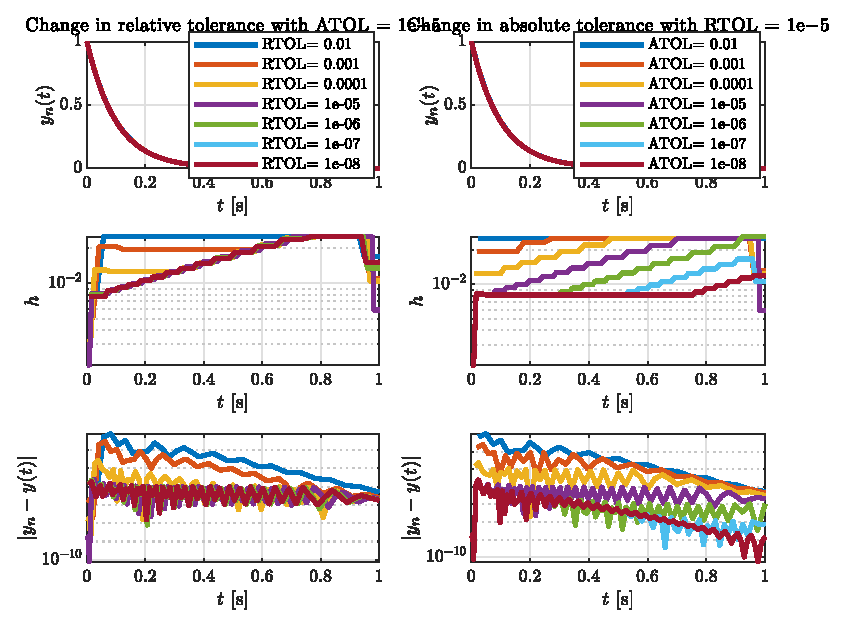
\includegraphics[width=\textwidth]{Figures/ode45_testCase.eps}
	\caption{Simulation of the test equation using the \textit{Dormand and Prince 4(5)} method with $\lambda=1$.}
	\label{fig:testode45}
\end{figure}
The consistency of the \textit{Dormand-Prince 4(5)} method is checked by using the same test equation that was used for the \textit{Euler forward} method. The test equation is given as follows:
\begin{align*}
	\textbf{Test equation: }f(t,y) &= -\lambda\,y, \quad y(0) = 1. & \textbf{Analytical solution: } & y = e^{-\lambda\,t}.
\end{align*}
Contrary to the fixed step method, the step length $h$ is varied throughout the simulation depending on the specified relative (RTOL) and absolute (ATOL) tolerances. 

The simulation results of the test equation are presented in \prettyref{fig:testode45}. From the figure, it is clear that by varying only the relative tolerance (RTOL), there is no significant difference in the error signal ($e(t_N) = |y_N - y(t_N)|$) at time $t = t_N$. This is because $h$ at $t = t_N$ for different RTOL are similar. However, varying the absolute tolerance (ATOL), it is clear that as $h\rightarrow0,\ |y_n - y(t)| \rightarrow0$. At time $t = t_{N-1}$ there is a sudden change in $h$ possibly be due to numerical rounding errors. Therefore time $t_{N-1}$ was considered for consistency check. According to the fundamental convergence theorem, the solver is convergent. Furthermore, from the figure it can be concluded RTOL controls the rate of change of $h$ and ATOL controls the absolute value of $h$

The average step size for convergence in the \textit{Dormand and Prince 4(5)} method have larger $h$ than the \textit{Euler forward} method. At the same time, the error in \textit{Dormand and Prince 4(5)} is lower than the error in the \textit{Euler forward}. This indicates the \textit{Dormand and Prince 4(5)} is a higher order method than the \textit{Euler forward}. 

\subsection{Motor equation}
\begin{figure}[t!b!]
	\centering
	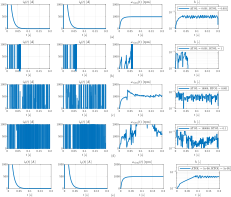
\includegraphics[width=\textwidth]{Figures/ef_MotorCase_ode45_Atol_Rtol.pdf}
	\caption{Simulation of the PMSM using Euler forward method with $\vd=\vq=800\,$V at different absolute (ATOL) and relative tolerances (RTOL). (a) ATOL = 0.001 RTOL = 0.001, (b) ATOL = 0.001 RTOL = 1, (c) ATOL = 1e4 RTOL = 0.001, (d) ATOL = 1e5 RTOL = 0.1, and (e) ATOL = 1e-8 RTOL = 1e-5}
	\label{fig:EMresOde45}
\end{figure}
\prettyref{fig:EMresOde45} presents the simulation results of a PMSM using the \textit{Dormand and Prince 4(5)} method. The figure shows the states (dynamic variables) \id, \iq and \wm as a function of time at different ATOL and RTOL. \prettyref{fig:EMresOde45}(a) presents the simulation results considering ATOL = RTOL = 0.001 and it is clear the dynamic variables \id, \iq, and \wm, converge implying the stability of both the ODE and the solver. Furthermore, the average set size is about 0.5e-3\,s and a deviation of 0.1e-3\,s. Moreover, at $t < 0.5$\,s the step size increases gradually from lower than 1e-4\,s to about 0.5e-3\,s. \prettyref{fig:EMresOde45}(b) presents simulation results with ATOL = 0.001 and RTOL = 1. From the figure it is clear that the simulation does not converter after $t \approx 0.05$\,s and the solutions is $\infty$. $h$ at $t_1$ (1\textsuperscript{st} step) is lower than 1e-4. However, just after a few steps, $h$ increases to 0.9e-3 as a consequence, the solver is does not converge. \prettyref{fig:EMresOde45}(c) and \prettyref{fig:EMresOde45}(d) presents simulation results with ATOL = 1e4 and RTOL = 0.001, and ATOL = 1e5 and RTOL = 0.1, respectively. From the figure it is clear that in both cases $h$ varies between 1e-4 and 1e-3\,s throughout the simulation and as a result, the simulation is although bounded, is not stable, ex: the drastic change in \wm at $t = 0.035$\,s indicates the instability of the solver. \prettyref{fig:EMresOde45}(e) presents simulation results with ATOL = 1e-8 and RTOL = 1e-5 and from the figure it is clear that the simulation converges. Furthermore, $h$ increases gradually to 0.5e-5\,s at $t = 0.75$\,s due to very low RTOL. 

%From the figure, although not straightforward, it can be seen that with lower $h\rightarrow0$ all the states converges to a constant value. This implies that that % the solver is 0\textit{-stable}. Furthermore, it is also clear that 
% the ODE system is stable for ATOL$\geq10$. 
%From the figure it is clear with lower $h\rightarrow0$. all the states converges to a constant value. This implies that that the solver is \textit{0-stable}. Furthermore, it is also clear that the ODE system is also stable. 
%
%In the previous section it was verified the \textit{convergence} of the numerical method. Therefore, it is observed that the simulated results with $h \leq 1\text{e}-4$ gives the a solution that is very close to the true solution to the ode system.

%the order of the system is calculated and presented in the table below:
%\begin{table}[h!]
%	\centering
%	\begin{tabular}{c|c|c|c}
%		TOL & $h_n$ & $|y_n - y(t)|$ & $p$ \\
%		\hline
%		0.1 & 0.07 & 5.82e-7 & \\
%		0.01 & 0.09 &5.89e-7 & 1.23\\
%		0.001 & 0.06 & 3.62e-7 & 1.02 \\
%		0.0001 & 0.06 & 8.18e-8 & 4.38\\
%		1e-5 & 0.03 & 9.37e-9 & 4.6 \\
%		1e-6 & 0.02 & 9.91e-10 & 6.67 \\		
%		1e-7 & 0.02 & 1.01e-10 & 9.13 \\
%	\end{tabular}
%\end{table}\\
%From the table and the figure, it is clear that, as $h\rightarrow0,\ |y_n - y(t)| \rightarrow0$. Therefore, according to the fundamental convergence theorem, the solver is convergent of order $p$. 
	% \newpage
	% \section{Conclusion}
A permanent magnet synchronous machine (PMSM) was modeled and simulated using a fixed-step method and a variable step-method
\subsection{Fixed-step method}
A simple \textit{Euler forward} numerical method was selected and the convergence of the solver was verified using a test equation. The PMSM was simulated between $ 0\leq t \leq 2$\,s for different step-lengths $h$. For $h \leq 1\times10^{-4}$\,s the solver is convergent. Using the definition of convergence, it is concluded that as $h\rightarrow0$, the numerical solution is close to the true solution of the ODE.
\subsection{Variable-step method}
A \textit{Dormand-Prince 4(5)} numerical method was selected and the convergence of the solver was verified using a test equation. The PMSM was simulated between $ 0\leq t \leq 2$\,s for different absolute (ATOL) and relative (RTOL) tolerances. For ATOL $\leq 10$ and RTOL $\leq 0.1$ the solver is both stable and the solution converges. Using the definition of convergence, it is concluded that as $h\rightarrow0$, i.e reducing ATOL and RTOL $\rightarrow 0$, the numerical solution is close to the true solution of the ODE.


%numerical solution gives the same solution as the differential equation. However, we cannot determine the solution analytically. Therefore, we need to try perform the several checks. The following sections cover these in detail. 
	% \newpage
	
%	Consistency
%	Whether or not the numerical solution gives the
%	same solution as the differential equation
%	Convergence
%	Whether the solution to the difference equations
%	becomes closer and closer to the solution of the
%	de for smaller and smaller step sizes
	
	
	\input{sections/simulation}
\end{document}